\documentclass[times, doublespace]{WileyNJD-v2}%For paper submission
%\documentclass[times]{simauth}
% Packages
%\usepackage{fcyheader}
\usepackage{mdframed}
%\usepackage{subcaption}
\usepackage{subfig}
\usepackage{url}
\usepackage{color}

%\usepackage[T1]{fontenc}
%\usepackage{times}
%\usepackage{bm}
%\usepackage{mathtime}

% Customised Commands
%\newtheorem{theorem}{Theorem}[section]
%\newtheorem{corollary}{Corollary}[theorem]
%\newtheorem{lemma}[theorem]{Lemma}
%\newenvironment{proof}[1][Proof]{\begin{trivlist}
%\item[\hskip \labelsep {\bfseries #1}]}{\end{trivlist}}
%\newcommand{\qed}{\nobreak \ifvmode \relax \else
%      \ifdim\lastskip<1.5em \hskip-\lastskip
%      \hskip1.5em plus0em minus0.5em \fi \nobreak
%      \vrule height0.75em width0.5em depth0.25em\fi}

% Bibliographystyle
\bibliographystyle{wileyj}

%\title{Statistical models for the source attribution of zoonotic diseases: A study of campylobacteriosis} 

\begin{document}
%\runninghead{Statistical models for the source attribution of zoonotic diseases}
%\author{Sih-Jing Liao\affil{a},
%Jonathan Marshall\affil{a}\corrauth\ \footnotemark[2], Martin L. Hazelton\affil{a} and Nigel P. French\affil{b}}
%\address{\affilnum{a} Institute of Fundamental Sciences-Statistics, Massey University, Palmerston North, New Zealand\\
%\affilnum{b} mEpiLab, Hopkirk Research Institute, Massey University, Palmerston North, New Zealand}
%\corraddr{Jonathan Marshall, Institute of Fundamental Sciences-Statistics, Massey University, Private Bag 11222, Palmerston North, New Zealand\\ \footnotemark[2] E-mail: J.C.marshall@massey.ac.nz}

\begin{abstract}

Preventing and controlling zoonoses with a public health policy depends on the knowledge scientists have about the transmitted pathogens. Modeling jointly the epidemiological data and genetic information on the cases provides a methodology for tracing back the source of infection. The genetic information on cases may be modelled at a variety of levels, as can the epidemiological data. In this paper, the attribution probability for human cases of campylobacteriosis for each source, conditional on the effect of the rurality of each case, is estimated utilising a model that incorporates genetic processes alongside a newly developed genetic-free model. We show that the inference from each model is comparable, and that the effect of rurality may be modelled linearly, with increasing rurality leading to increasing likelihood of ruminant-sourced campylobacteriosis.
  
\end{abstract}
%\keywords{source attribution; \textit{Campylobacter}; multinomial model; Dirichlet prior; HPD interval; DIC}

%\maketitle

\section{Introduction}
Modeling of disease surveillance data to explore patterns of infectious diseases has had a long history in public health. Infectious diseases can cause high economic and medical costs due to morbidity and mortality. In recent decades, the annual number of global deaths caused by infections has leveled off at approximate 15 million and may remain at this level for the next three decades \cite{DyeC, WHOM}. In order for such an enormous health burden to be reduced, preventing and controlling infectious diseases becomes extraordinarily important, which depends on how much we know about the course of disease transmission. For zoonotic diseases, where transmission to humans from animal reservoirs may be via food, water, through environmental contamination or via direct contact with animals, knowledge of the potential sources and pathways of infection is key in improving understanding of the burden of disease. Quantifying the burden of illness to each pathway and source, provides valuable information to health professionals making decisions on public health policy for disease control. 

Over the last few decades there have been many models developed for the analysis of zoonotic diseases. Epidemiological models make use of the incidence of cases and geographic data to capture the main characteristics of disease spread. For example, the Susceptible-Infectious-Recovered model \cite{Kerm} classifies populations into a susceptible, infective and recovered status enabling an estimation of the number of individuals who are likely to be infected. Also, models with a combination of spatial and temporal data enable the prediction of the time frame and areas where a disease outbreak is likely to occur \cite{HeldL, Hoehl, Simo}. However zoonotic transmission from animals to humans may be complex, involving many sources and exposures linked by differing pathways. For instance, infected wild birds may contaminate environmental water and cause disease spread to water users, either humans or other animals \cite{Wagen}. Tracing the source of infection is thus crucial to increasing the ability to implement risk management and intervention \cite{Wilso, Morel}. In terms of statistical analysis, modelling zoonoses requires an advanced approach with the focus changed from just epidemiology to a combination of epidemiology, evolutionary genetics and biology \cite{Muell}. Hence, some source attribution models have been proposed to estimate the number of cases attributable to different sources by utilizing epidemiological information and the association with genotypes found in humans and sources \cite{vanP, Hald, MullA}. 

\begin{table}
  \begin{center}
    \begin{tabular}{crrrrrrr}
      \toprule
      ST & \textit{asp} & \textit{gln} & \textit{glt} & \textit{gly} & \textit{pgm}& \textit{tkt}& \textit{unc}\\ \midrule
      45  & 4 & 7 & 10 & 4 & 1 & 7 & 1\\
      474 & 2 & 4 & 1 & 2 & 2 & 1 & 5 \\
      \bottomrule
    \end{tabular}
  \end{center}
  \caption{The allelic profile of genotypes ST-45 and ST-474 is composed of seven allele numbers at each of the seven loci.}
  \label{tab0}
\end{table}

The genetic information used in such integrated models is typically through genotyping that groups closely related organisms together to capture broader changes in DNA occurring in the transmitted pathogens \cite{Cotta}. Typically molecular typing methods, such as multilocus sequence typing (MLST) \cite{Dingl, Coll} might be used, which utilises nucleotide sequences of internal fragments of a small set of housekeeping genes. Such sequences have sufficient variation to distinguish differing pathogen lineages, while being relatively stable within lineages. Each unique nucleotide sequence (allele) at each housekeeping gene (loci) is assigned a number, and the set of numbers across all loci (the allelic profile) is then taken as the genotype, with is usually also assigned a number.

For the pathogen \textit{Campylobacter} which causes campylobacteriosis, a worldwide gastrointestinal disease in humans, the MLST scheme consists of housekeeping genes \textit{asp}A (aspartase A), \textit{gln}A (glutamine synthetase), \textit{glt}A (citrate synthase), \textit{gly}A (serine hydroxymethyltransferase), \textit{pgm} (phosphoglucomutase), \textit{tkt} (transketolase), and \textit{unc}A (ATP synthase $\alpha$ subunit). An illustrative example of MLST data for \emph{Campylobacter jejuni} is presented in Table~(\ref{tab0}). It shows that the genotypes ST-45 and ST-474 have different allelic combinations across the seven loci. The different allelic profiles enable comparison of gene similarities or dissimilarities so that an association between sources and infected cases can be made, by comparing the distribution of genotypes from human cases with those from potential reservoirs.

The first step for attribution models that utilise genetic information is building the sampling distribution of genotypes among each putative source. This may range from using the proportion of each observed genotype (CITATION: TINA HALD) on each source through to utilising allelic profile information to derive mutation and recombination rates within each source, and migration rates between each source (CITATION: ISLAND MODEL). A key question is whether more complex genetic models yield superior attribution results or whether a significantly simpler model may suffice, however few authors in the literature have addressed this point. This becomes more important as model complexity extends to include epidemiological covariates. We are therefore motivated to develop a simple genetic model in order to assess the additional information that the more complex models provide.

In this paper we develop statistical models for the source attribution, and use a case study of human campylobacteriosis conducted in New Zealand \cite{Marsh} as a demonstration. Human campylobacteriosis is caused by \textit{Campylobacter}, of which \textit{C. jejuni} and \textit{C. coli} are the dominant species associated with 80\% and approximately 15\% of illnesses, respectively \cite{Guert}. The common symptoms of infection are diarrhea, abdominal pain and fever. However, a severe complication named Guillain Barre syndrome may develop, which is a life-threatening disease that weakens the nervous system and leads to paralysis in limbs and respiration \cite{Hanha}. The pathogen can be spread between animals, or from animals and wild birds to humans. The transmission route can be via drinking contaminated water, eating undercooked animal food products, or handling animal food products that are already contaminated by faeces. In this study, we compare the performance of the asymmetric Island model \cite{Wilso}, which considers genetic evolution when estimating the genotype sampling distribution on each source, to a simple model that utilises only the prevalence of each type to derive the sampling distribution. We then extend both models to incorporate covariates, exploring the effect of human case rurality on attribution results, modelling attribution by rurality using a linear trend or using separate categories in a Bayesian context, and performing model comparison.

\section{Models for source attribution with and without information of evolutionary change}
\subsection{Notation and assumptions}
The ultimate goal of attribution models is to estimate the probability that the observed human cases arise from each putative source. Given genotyping information, we first estimate the sampling distribution of genotypes for each source, and then estimate the appropriate combinations of those genotype distributions that most likely give rise to that observed among human cases. Specifying first the sampling distribution of genotypes found on sources is fundamental for the purpose of not only exploring how it affects the source attribution probability, but also investigating the difference in attribution effect made between the model with genetic information and the model without it.

Suppose we have isolates collected from human and non-human cases, of which $H$ isolates belong to humans, and the remaining $N$ isolates are categorized in $J$ groups as the major sources attributed to the infection. Let $I$ genotypes be the total number of unique STs detected from all isolates, and denote $n_j$ as the marginal frequency of STs found in source $j$, where $\sum_j^J n_j = N$. Typically, the number of detected STs $I$ is smaller than the sample size of isolates as multiple isolates will be of the same type.

The likelihood of observing human cases with types $\text{ST}_1, \text{ST}_2, \ldots \text{ST}_H$ follows a multinomial distribution, which via the law of total probability may be expressed as
\begin{align}
  L\Big(\text{ST}_1, \text{ST}_2, \ldots, \text{ST}_H\Big)=\prod_{h=1}^{H}\sum_{j=1}^{J} p\Big(\text{ST}_h \vert \text{source } j\Big) p(\text{source }j),
  \label{Olikh}
\end{align}
where $p(\text{ST}_h \vert \text{source }j)$ is the probability that $\text{ST}_h$ arises from the sampling distribution of source $j$, $p(\text{source }j)$ is the attribution probability that a random human case is infected from source $j$. Given we know $p(\text{ST}_h \vert \text{source }j)$, estimation of $p(\text{source }j)$ may be found by optimising the likelihood \ref{Olikh}, for example using a Metropolis Hastings algorithm within a Bayesian context, with suitable priors on $p(\text{source }j)$.

The asymmetric Island model \cite{Wilso} adopted in the source attribution study for human campylobacteriosis \cite{Marsh} utilises the allelic profile information for each genotype in an evolutionary model, estimating mutation and recombination probabilities within, and migration probabilities between, each source `island'. It thus estimates $p(\text{ST}_h \vert \text{source }j)$ indirectly, by first estimating the evolutionary parameters, and then deriving the sampling distributions. This allows the asymmetric Island model to estimate the likelihood of observing a genotype on a source when it has not been previously observed.

To discover the effect of incorporating genetic information at the allelic profile level as used in the island model, a simple model is developed for the genotype sampling distribution. With the assumption that the observed distribution of genotypes is representative of the true distribution, we model observed genotypes using a multinomial distribution. Let $x_{ij}$ denote the count of ST-$i$ found in source $j$ with the probability $\pi_{ij}$, where $i=1, \ldots, I$ and $j=1, \ldots, J$. To make inference about $\pi_{ij}$, the likelihood is of a multinomial form,
\begin{align}
        L(\boldsymbol{\pi}_{j} ; \boldsymbol{x}_{j}) & = \frac{n_j!}{\prod_{i=1}^{I} x_{ij}!} \prod_{i=1}^I \pi_{ij}^{x_{ij}}, \notag
\end{align}
where $x_{ij}$ can be $0$, indicating STs are yet observed on the sources; $n_j=\sum_{i=1}^I x_{ij}$ is the total count of ST found on source $j$ and $\pi_{ij}$ is subject to $\sum_{i=1}^I \pi_{ij} =1$, and $0 \leq \pi_{ij} \leq 1$. As the family of Dirichlet distributions is a conjugate pair for the multinomial distribution, assume the prior for $\boldsymbol{\pi}_{j}$ follows a Dirichlet density with parameters $\boldsymbol{\alpha}_{j}$,
\begin{align}
  p(\boldsymbol{\pi}_{j}) & \propto \prod_{i=1}^{I}\pi_{ij}^{\alpha_{ij}-1}. \notag
\end{align}

Then the posterior for $\boldsymbol{\pi}_{j}$ takes the form of a Dirichlet probability function with parameters $(\boldsymbol{\alpha}_{j}+\boldsymbol{x}_{j}-\boldsymbol{1})$,
\begin{align}
        p(\boldsymbol{\pi}_{j} \vert \boldsymbol{x}_{j} ) & \propto L(\boldsymbol{\pi}_{j} ; \boldsymbol{x}_{j}) p(\boldsymbol{\pi}_{j}) \notag \\ 
       & \propto \prod_{i=1}^{I}\pi_{ij}^{\alpha_{ij} + x_{ij}-1}, \quad \alpha_{ij} >0. \notag
 \end{align}

To express the belief that every isolate is equally likely \emph{apriori}, the parameter of the Dirichlet prior is assumed as $\boldsymbol{\alpha}_{j}=\boldsymbol{1}$. Therefore, p(ST $i\vert$source $j$, $\boldsymbol{X}$) can be obtained by simulating from the Dirichlet posterior.

Lastly, the overall likelihood can be computed by substituting the respective sampling distribution from the island model and the simple model for $p(\text{ST }i(h)\vert\text{source }j)$ in equation~(\ref{Olikh}), and integrating over the posteriors.

TODO: JM: I think including an algorithm here might be useful. It could then be extended in section 3.1


\subsection{Campylobacteriosis data}

The source attribution study used here has MLST data collected in the Manawatu region of New Zealand from 2005 to 2014. The sampling has been done in the same time and from the same geographical location that gives 3,480 isolates taken from human and non-human cases, 1,400 of which are from humans. The non-human isolates are sampled from cattle, sheep, wild birds, environmental water and chicken carcasses, and we therefore put them into four groups of major source of infection: poultry, ruminant, water and others. The total number of unique ST typed from all isolates is 355, and 35\% of genotypes are found among human cases. Table~(\ref{tab1}) lists five common genotypes typed in human and source isolates. The first four genotypes are frequently observed in human cases. For four sources, ST-45 and ST-474 are commonly detected in poultry, while ST-42 and ST-61 are typically found in ruminants. Some studies also discover that human cases with ST-45 or ST-474 are likely attributable to poultry, whereas human cases with ST-42 or ST-61 are more likely attributable to ruminants \cite{Muell, Coll, Cart}. Furthermore, it also shows that there are no observations of ST-2381 in humans, poultry or ruminants, indicating that the genotype may only appear in the water or other sources.

The data also contain location variables such as a binary variable specifying whether a typed human case is from urban or rural areas, and a categorical variable further splitting up the areas into seven levels: highly rural/remote area, rural area with low urban influence, rural area with moderate urban influence, rural area with high urban influence, independent urban area, satellite urban area and main urban area. Figure~(\ref{fig1}) presents the number of typed human cases living either in urban or rural areas between 2005 and 2014. It shows that the number of typed cases in urban areas was more than that in rural areas, particularly from 2005 to 2007, then it dropped in 2008 and rose up steadily in the following years. The results are from an intervention in the poultry industry implemented by the New Zealand Food Safety Authority (NZFSA) in 2007 and 2008. Table~(\ref{tab2}) further lists the number of typed human cases in each classification of rurality. The degree of rurality is a set of integers with a range of [-3,3] corresponding to each defined geographical level. Overall, the table tells us that more than 70\% of typed cases lived in urban areas, and approximately 7.5\% of individuals have no information about the location. We will neglect the missing data in the following analysis by assuming that these cases are randomly missing. Also, as 2006 Census Meshblock Dataset pointed out \cite{Stat}, the total number of dwellers living in urban and rural areas in the Manawatu region was 130,962 and 20,337, respectively. Suppose the population size in the region during 2005 and 2014 is constant, the case rates of the two areas in 2006 are similar with about 0.12\%, this then implies that more cases found in urban areas is simply because more residents are living there. After the intervention, the rate in rural areas still stays at the same level, but the rate in urban areas remarkably decreases. 


\begin{table}
  \begin{center}
    \begin{tabular}{crrrrr}
      \toprule
      ST & Human & Poultry & Ruminants & Water & Others\\ \midrule
      42 & 54 & 7 & 52 & 10 & 2\\
      45  & 141 & 154 & 10 & 21 & 54\\
      61 & 64 & 7 & 54 & 2 & 1\\
      474 & 239 & 60 & 15 & 5 & 7\\
      2381 & 0 & 0 & 0 & 21 & 3\\
      \bottomrule
    \end{tabular}
  \end{center}
  \caption{The frequency of five genotypes found from human and four source isolates.}
  \label{tab1}
\end{table}

\begin{figure}
\centering
%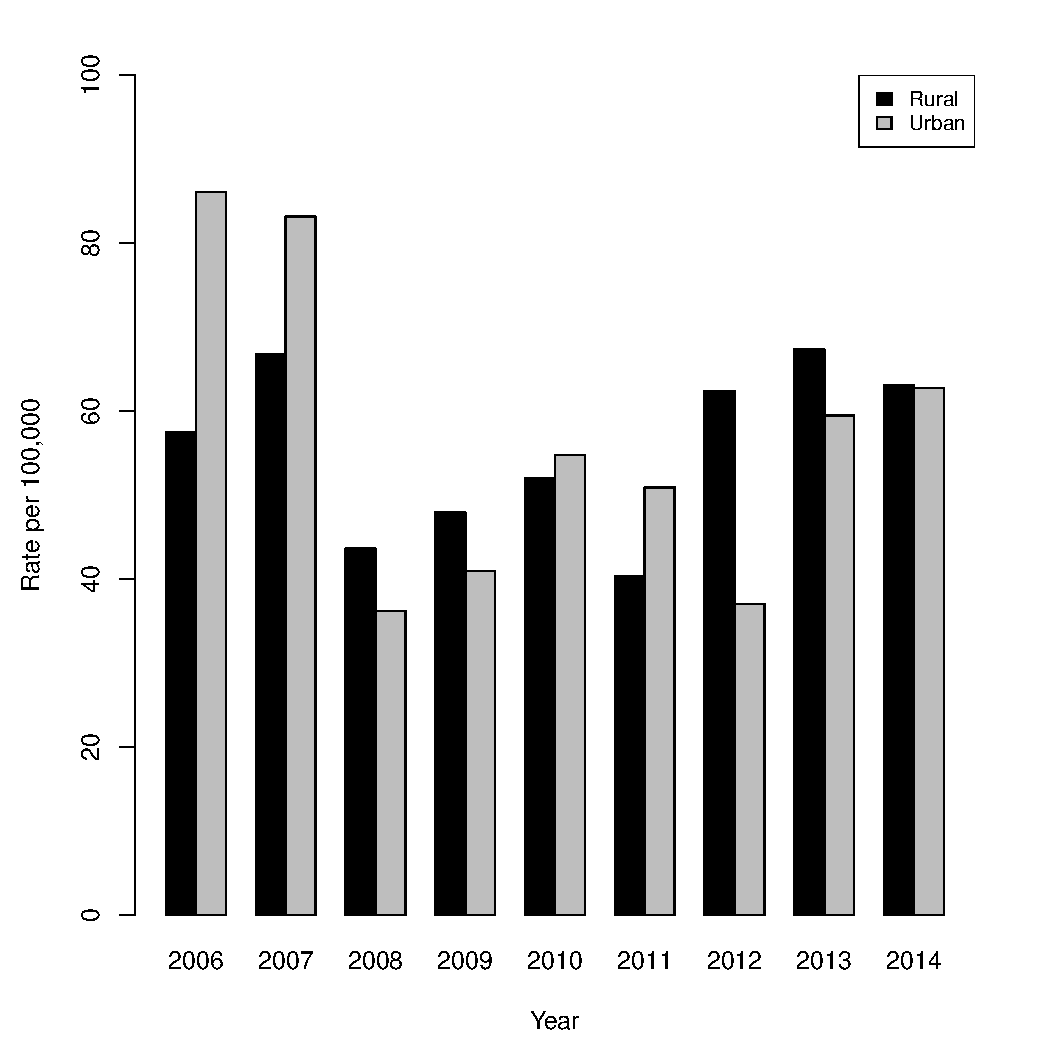
\includegraphics[width=.5\linewidth]{Figures/Databar}
\caption{The number of typed human cases coming from urban/rural areas in the Manawatu region of New Zealand during 2005 and 2014. A poultry intervention conducted in 2007 and 2008 resulted in a decreasing incidence of campylobacteriosis in the following two years in urban areas.}
\label{fig1}
\end{figure}

\begin{table}
  \begin{center}
    \begin{tabular}{rlrr}
      \toprule
      Rurality scale & Description & Typed human cases & Population in 2006\\ \midrule
      -3 & Highly rural/remote area & 19 & 1,572\\
      -2 & Rural area with low urban influence & 92 & 8,373\\
      -1 & Rural area with moderate urban influence & 127 & 10,392\\
      0 & Rural area with high urban influence & 70 & 6,579\\
      1 & Independent urban area & 230 & 28,611\\
      2 & Satellite urban area & 178 & 19,725\\
      3 & Main urban area & 579 & 76,047 \\
      \bottomrule
    \end{tabular}
  \end{center}
  \caption{The number of human cases typed during 2005 and 2014 in the Manawatu region of New Zealand whose location fell in each grade of rurality corresponding to the defined area against the respective total number of residents in 2006. In general, the scales that ranged between 0 and 3 are regarded as the urban areas and the remaining scales belong to the rural areas.}
  \label{tab2}
\end{table}

\section{Model fitting for source attribution on rurality scale}
The island model and the simple model in the preceding section describe the distribution of STs by integrating with or without genetic variations in DNA sequences respectively. To further estimate the attribution probability a source contributes the infection to human beings, let $F_{jh}$ denote the attribution probability of source $j$ for the h$^{th}$ human case, with constraints $\sum_{j=1}^J F_j =1$ and $0 \leq F_j \leq 1$, where $j=1, \ldots, J$. We model the probabilities $F_{jh}$ using a linear model on the logit scale, that is,  

\begin{align}
  F_{jh}  = \frac{\exp (f_{jh})}{\sum_{j=1}^4 \exp(f_{jh})},
  \label{capF}
\end{align}

where $f_{4h}=0$ is treated as the baseline of $f_{jh}$. Consider the case where the data comprise of $H$ human cases, and with the associated assigned STs and $p$ variables, we develop a general model of $f_{jh}$ with linear combinations of the variables, $c_1, \ldots, c_p$. The model for the h$^{th}$ individual is then of the form,

\begin{align}
f_{jh}  = \alpha_{j} + \beta_{j1} c_{1h} + \beta_{j2} c_{2h} + \ldots + \beta_{jp} c_{ph},  \notag   
\end{align}

so that more covariates can be considered in the model to further investigate how the attribution is associated with the factors of interest.

To apply the general model of $f_{jh}$ to the campylobacteriosis data, assume $z$ is the categorical variable representing the classified location of each human case. Then two approaches of treating the variable $z$ in model fitting are proposed: one is to treat it as numeric, and the other as categorical. To differentiate the performance between the two fitted models, we link ``the linear model'' and ``the categorical model'' to the first and the latter fitted model, respectively. Hence, the linear prediction function for source $j$ for each human case given the degree of rurality is a numeric variable and can be written as,

\begin{align}
  f_{jh} = \alpha_{j} + \beta_{j} z_{h},
  \label{modL}
\end{align}

where $z_{h}$ can be any number of the seven scales if case $h$ was from such a degree of rurality. Conversely, if we treat each of the seven rurality degrees as an indicator with a superscript number $d$, which corresponds with the position of the category ranged from -3 to 3, the model~(\ref{modL}) can be rewritten as,

\begin{align}
  f_{jh} & = \beta_{1j} z_{1h}+ \beta_{2j} z_{2h} + \ldots + \beta_{dj} z_{dh} + \ldots +  \beta_{7j} z_{7h}, \\
  \text{where} & \notag\\
z_{dh} & =
\left\{\begin{array}{rcl}
1 && \mbox{if case $h$ is in the category $d$,} \notag \\ 0 && \mbox{otherwise}. 
\end{array}\right.
  \label{modC}
\end{align}

As a consequence, the estimated attribution probabilities are obtained via equation~(\ref{capF}) after fitting the data to model~(\ref{modL}) or to model (4).

\subsection{MCMC algorithm}
In the interest of quantifying the uncertainty of the posterior attribution probability, the Markov chain Monte Carlo (MCMC) method is applied. Assume the priors on parameters of interest in model~(\ref{modL}) and model (4) follow a standard normal distribution. Denote $\boldsymbol{\theta}$ as a parameter set of $\theta_{(t)}$, where t indicates the t$^{th}$ order of parameters in the model, $t=1, \ldots, T$, namely, either $(\alpha_1, \alpha_2, \alpha_3, \beta_1, \beta_2, \beta_3)$ in model~(\ref{modL}) or $(\beta_{11}, \beta_{12}, \ldots, \beta_{dj}, \ldots, \beta_{73})$ in model (4). We use the Metropolis-Hastings algorithm to update $\theta_{(t)}$ and hence $f_{jh}$, and $ F_{jh}$ in a Markov chain with a length of 30,000 iterations. With the aim of the chain convergence, the first 5,000 samples are removed and the sequence is thinned every 10$^{th}$ sample. Here are the steps in detail:

\begin{enumerate}

\item Sample $T$ random values from $N(0,1)$ as starting points of the parameter set $\boldsymbol{\theta}$ for model~(\ref{modL}) or model (4) 

\item Propose a candidate $\boldsymbol{\theta}^*$ with one $\theta_{(t)}$ updated by a normal proposal distribution, $N(\theta_{(t)}, 1)$

\item Use $\boldsymbol{\theta}^*$ to calculate a new set of $f^*$ for source $j$, $j=1, 2, 3$, via model~(\ref{modL}) or model (4), and find the associated $F^*$ for each case by putting the vector $(f^*, f_4=0)$ in equation~(\ref{capF}) 
  
\item Compute the acceptance rate $\alpha$, a product of the likelihood ratio, the proposal ratio and the prior ratio, given by,

\begin{align*}
\frac{L\Big(F^*; \text{ST}, \boldsymbol{Z}\Big)}{L\Big(F; \text{ST}, \boldsymbol{Z}\Big)}\frac{Q\Big(\theta_{(t)} \vert \theta_{(t)}^*\Big)}{Q\Big(\theta_{(t)}^* \vert \theta_{(t)}\Big)}\frac{p\Big(\theta_{(t)}^*\Big)}{p\Big(\theta_{(t)}\Big)}, 
\end{align*}

where the likelihood $L\Big(F^*; \text{ST}, \boldsymbol{Z}\Big)$ involves the rurality covariate $\boldsymbol{Z}$ resulting from the attribution probability, $p(\text{source }j\vert \boldsymbol{Z}$) with an assumption that the genotype distribution on sources is independent of the covariate. Then, a random value of $u$ is generated from $U(0,1)$. If $\alpha$ meets $u < \min \left\{1, \alpha \right\}$, in the next state the current proposals of $f^{(*)}$, $F^{(*)}$ and $L\Big(F^{(*)}; \text{ST}, \boldsymbol{Z}\Big)$ are updated; otherwise, the previous proposals are retained. 
\end{enumerate}

%KEEP IT IN .TEX AND ADD IT AS COMMENTS IN YOUR CODE. The above function can be equivalently written as a product of the likelihood ratio and the prior ratio due to an assumption of the symmetric proposal function $Q$ resulting in $\frac{Q(\theta_{(t)} \vert \theta_{(t)}^*)}{Q(\theta_{(t)}^* \vert \theta_{(t)})}=1$. For the prior ratio in the later part of above function, we can obtain by calculating,

%\begin{align*}
%\frac{p(\theta_{(t)}^*)}{p(\theta_{(t)})} & =\frac{\frac{1}{\sqrt{2\pi\sigma^2}}\exp (-\frac{1}{2}\frac{\theta_{(t)}^*^2}{\sigma^2})}{\frac{1}{\sqrt{2\pi\sigma^2}}\exp (-\frac{1}{2}\frac{\theta_{(t)}^2}{\sigma^2})}\\
%& = \exp\Big(\frac{\theta_{(t)}^2-\theta_{(t)}^*^2}{2\sigma^2}\Big).
%\end{align*}

\section{Results}

\begin{figure}
\centering
%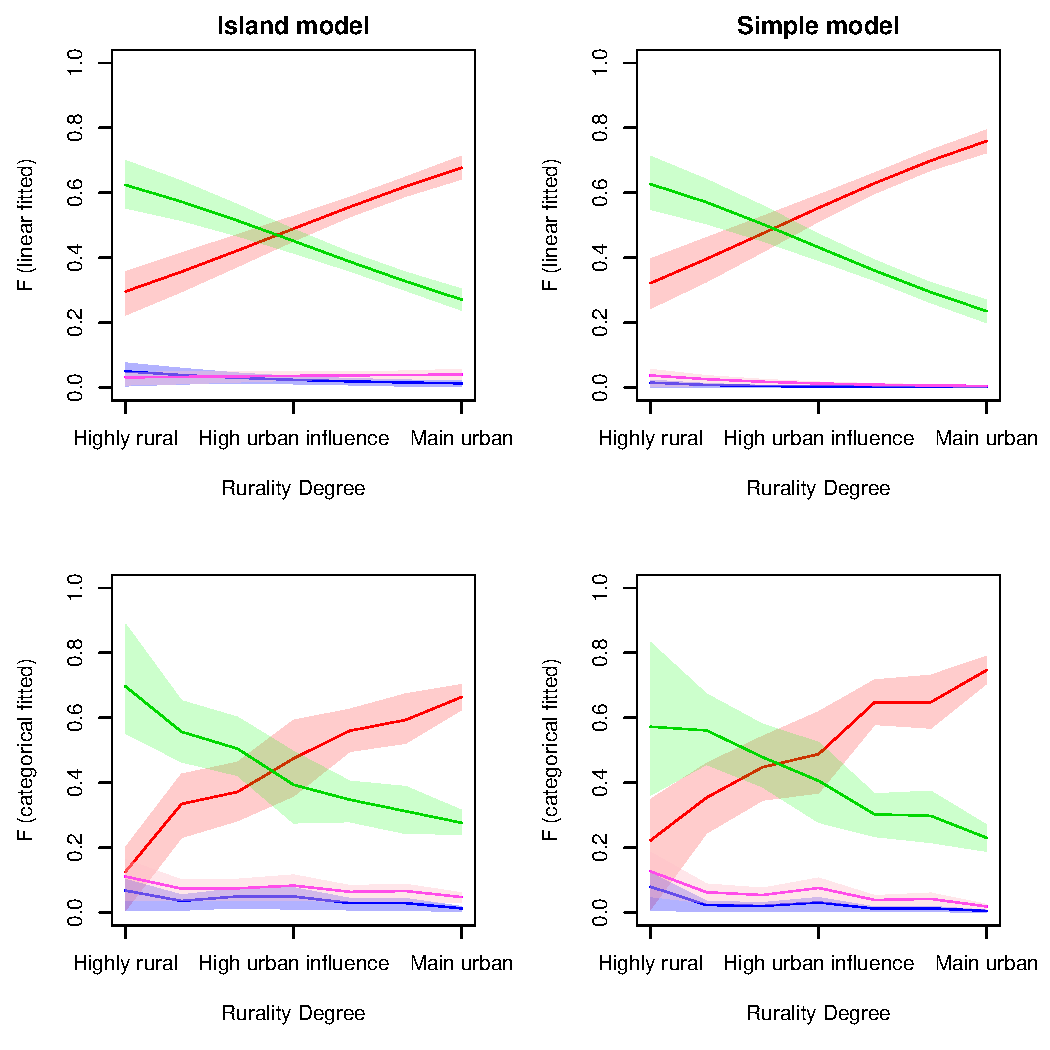
\includegraphics[width=.9\linewidth]{Figures/FCILandC(5)}
\caption{The posterior mean of samples $F$ with 80\% HPD interval for source: poultry (red), ruminants (green), water (blue) and others (pinks) over the rurality degrees. The samples of attribution probability are generated from the two respective fitted models: the linear model (upper panel) and the categorical model (lower panel), given the sampling distribution of genotypes with evolutionary information (the island model) or without any genetic information (the simple model).}
\label{fig2}
\end{figure}

\begin{figure}
\centering
%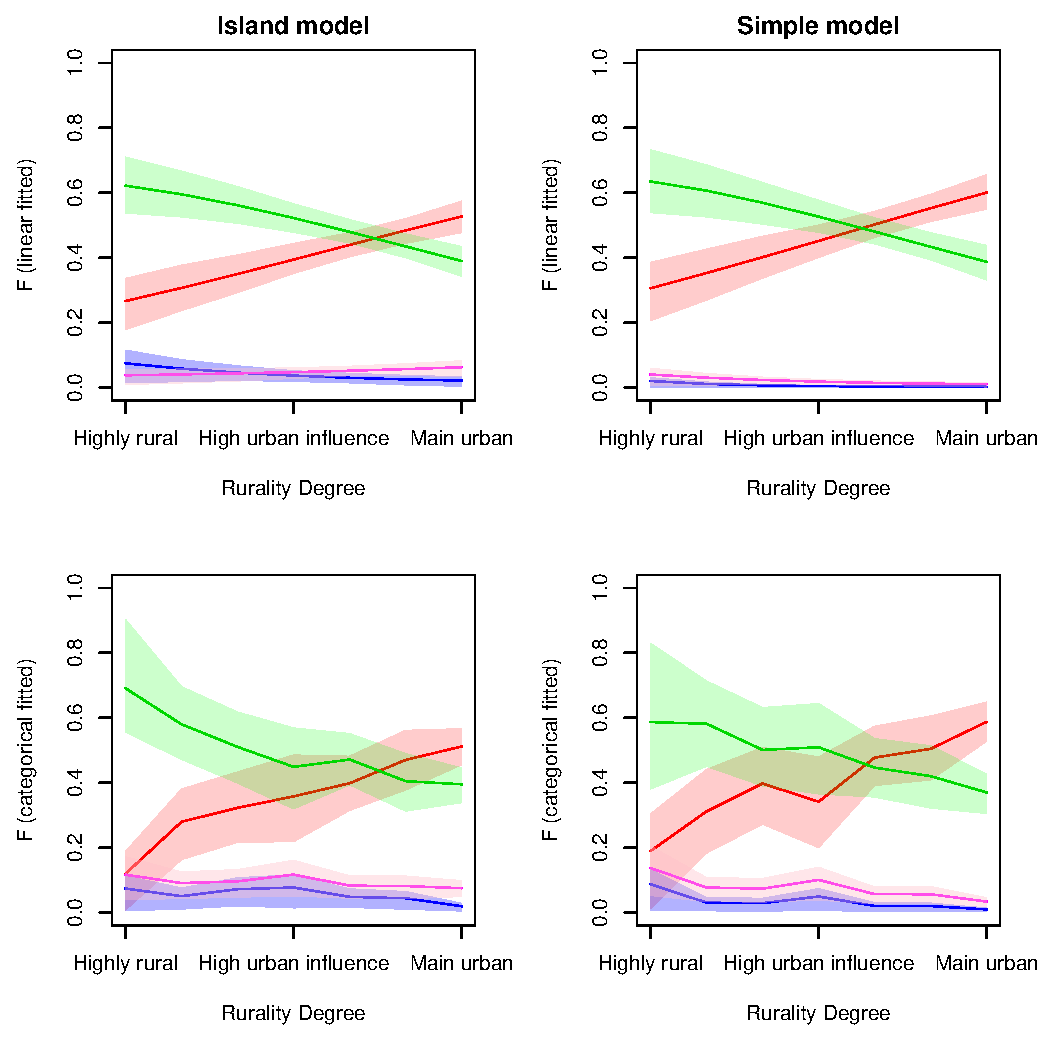
\includegraphics[width=.9\linewidth]{Figures/FCILandC(8)}
\caption{The posterior mean of samples $F$ with 80\% HPD interval for four sources over seven rurality categories after applying our methods to data with the post-intervention time period from 2008 to 2014. The samples of attribution probability are generated from the two respective fitted models -- the linear model (upper panel) and the categorical model (lower panel) -- given the genotype distribution based upon the island model or the simple model.}
\label{fig3}
\end{figure}

To investigate the association between source attribution and human infection, we apply the methods demonstrated in the preceding sections to the campylobacteriosis data and also rearrange the data frame from the ST-based structure to the case-based one for model fitting. The posterior mean of samples $F$ with the 80\% highest posterior density (HPD) interval for each source is illustrated on each rurality grade in Figure~(\ref{fig2}). Given different genotype distributions, the upper panel of the figure is based on the linear model, whereas the lower panel is generated from the categorical model.

%80% credible interval can be 10th through 90th percentile (central credible interval) or highest posterior intervals where 80% is picked that minimises length
%
For the linear model, the simple model suggests a slightly higher attribution probability for poultry and a little decreased probability for ruminants in main urban areas, compared to what the island model estimates. Also, the 80\% HPD interval of $F$ for poultry and for ruminants based on the simple model seems marginally wider than that for the island model. So, there is no significant difference in the proportion of human cases attributed to each source between the island and the simple models. For the categorical model, the comparison between the island and the simple models is quite similar to that for the linear model except for the distinguishable attribution for poultry and ruminants in highly rural areas and the much wider credible intervals of $F$ for four sources. For the two fitted models, the narrower credible intervals noticed in very rural areas from the island model might indicate that the island model gives a little more accurate sampling distribution for poultry and ruminants genotypes especially typed in humans living in rural areas. Further, the relatively larger credible intervals observed in the categorical model might be the effect of allocating the number of cases to each qualitative scale (as a dummy variable), particularly in rural areas due to small observations.

As is known, poultry is the major cause of human campylobacteriosis in urban areas \cite{MullA, Marsh, MullM}. Figure~(\ref{fig2}) shows further evidence that poultry starts becoming the dominant source contributable to the infection from places between minor rural and minor urban areas. In contrast, ruminants are becoming the most attributable source when locations are getting farther away from rural areas with a moderate urban influence. As to water and other sources, they seem to be less influenced by the rurality levels because the probabilities remain less than 0.2 over the seven categories.

Moreover, with a view to examining the robustness of our results, the approach is also applied to data with the time period of post-intervention from 2008 to 2014. The source attribution at different rurality levels is then illustrated in Figure~(\ref{fig3}), displaying that the overall attribution over four sources is moderately consistent with the patterns we previously discovered. However, Figure~(\ref{fig3}) shows a marked decline of attribution probability for poultry and a small rise in probability for ruminants in main urban areas. Despite the fact that the intervention did not eliminate the infection arising from poultry \cite{MuelM}, the reduction highlights the significant improvement in contribution of poultry to the disease, particularly in urban areas where most cases lived. This finding also accords with what Sears A. and other researchers investigated for the effect on poultry intervention \cite{AnnS}. 

Last, we use deviance information criterion (DIC) to evaluate if the linear model or the categorical model is more suitable to describe the data with different time periods of study. Given the sequence type information from the island model and the simple model, Table~(\ref{tab3}) compares the DIC values of the linear model to that of the categorical model, applied to data with the whole period of study and to data with the post-intervention time period. It tells that the linear model always performs better than the categorical model as this model is penalized more in DIC due to the larger number of parameters. This shows that the assumption of a linear effect on the rurality scales against the source attribution is reasonable. 

\begin{table}
  \begin{center}
    \begin{tabular}{crrrrr}
      \toprule
      & \multicolumn{2}{c}{Island model}  & \multicolumn{1}{c}{} & \multicolumn{2}{c}{simple model} \\
      %&  \cmidrule(lr){2-3}\cmidrule(lr){5-6} 
      Data & Linear & Categorical & & Linear & Categorical\\ \midrule
      whole period  & 7913.6 & 7943.3  & & 10328.4  & 10389.8 \\
      post-intervention period  & 5413.4  & 5439.5  & & 6615.1   & 6668.9 \\
      \bottomrule
    \end{tabular}
  \end{center}
  \caption{DIC values for the linear model and for the categorical model applied to the data from 2005 to 2014 (whole period) and to the data from 2008 to 2014 (post-intervention period) given the genotypic information is from the island model or the simple model.}
  \label{tab3}
\end{table}

\section{Discussions}
In recent epidemiological literature, modeling for zoonotic diseases with genomic data has commonly emerged that provides an added value to unravel the transmission of pathogens, but increases difficulties in analytically assessing models. In this paper, with an application of a campylobacteriosis study, we not only compare the source attribution based on the genotype distribution with or without pathogenic evolutionary information, but also unfold the infection attributable to sources at different geographical levels. 

In light of the different estimates of sampling distribution of genotypes from the island and the simple models, two approaches of model fitting (linear and non-linear) are utilized to estimate the attribution probability via the Matropolis-Hastings algorithm. The estimate of attribution probability $F$ is not straightforward as it is on a logit scale. To examine how the values of $f$ affect the attribution probabilities, we change the standard deviation of the prior distribution from 1 to 2 in the algorithm. It turns out that the associated posterior mean of $F$ for each source is invariant despite the fact that the proposals of $f$ jump even wider in the random walk. This is because the denominator of the transformation equation~(\ref{capF}) balances the impact made by $f$. Further, a linear model is applied to fit the data, assuming the relationship between the predictor and the response variable is linear. This assumption is also in some way supported by the results produced by the categorical model as it displays a linear-like pattern, illustrating how the level of rurality affects the attribution probability. 

This study can contribute considerably to the assessment of the final inference made between the models considered with and without the genetic information. The source attribution estimated by the linear and the non-linear models agrees fairly given two different genotype distributions, indicating that the simple model can at least do similar work to the island model. Also, the extension of the developed model fitting for this application is attainable. There are two possible directions: the genetic data, which will become more comprehensive due to rapidly evolving molecular tools, and the role of water source.

Concerns about the water source have been recently raised \cite{Wagen}. Water plays an important role in the transmission network that can disperse pathogens to uninfected users such as humans, wild birds and livestock over wide areas \cite{Cart, Skel, Leve, Case}. But, water is unlike hosts providing a physical environment to pathogens evolving and amplifying; it is simply a medium storing pathogens that come from infected users, and passes them to the next users who are yet to be infected. Hence, excluding water as a source of infection and discovering a better way to consider it in the extended model will be one of the next steps. Furthermore, a novel MLST approach, whole-genome MLST (wgMLST), has recently appeared in the literature \cite{Bigg, Kova, Llar}. The wgMLST method considers more than 1,000 loci enabling the investigation of the association between isolates with identical allelic profiles and the common source of infection. The new genotyping approach overcomes the limit of the traditional MLST method that only captures genetic diversity on seven loci \cite{Bigg}. This means that how to select invaluable information from such large data, and how to develop a sophisticated model to fit the well-filtered data, will be two potential challenges in future research.


\section*{Acknowledgements}
% We would like to thank two anonymous reviewers for their helpful comments and suggestions, which have led to an improved version of the paper.

%\appendix
%\section{Appendix A}

\bibliography{BibArt}
\end{document} 
